\noindent The diagram seen in figure \ref{fig:Polite-Mobile-Obstacle-Avoidance-Flowchart} illustrates the software logic flow for our system. \\

\noindent The flowchart begins at processing the Sonar sensor readings. These readings are done first due to their relatively low latency and accuracy for determining if we are in need of an immediate stop.  \\

\begin{figure}[H]
	\centering
	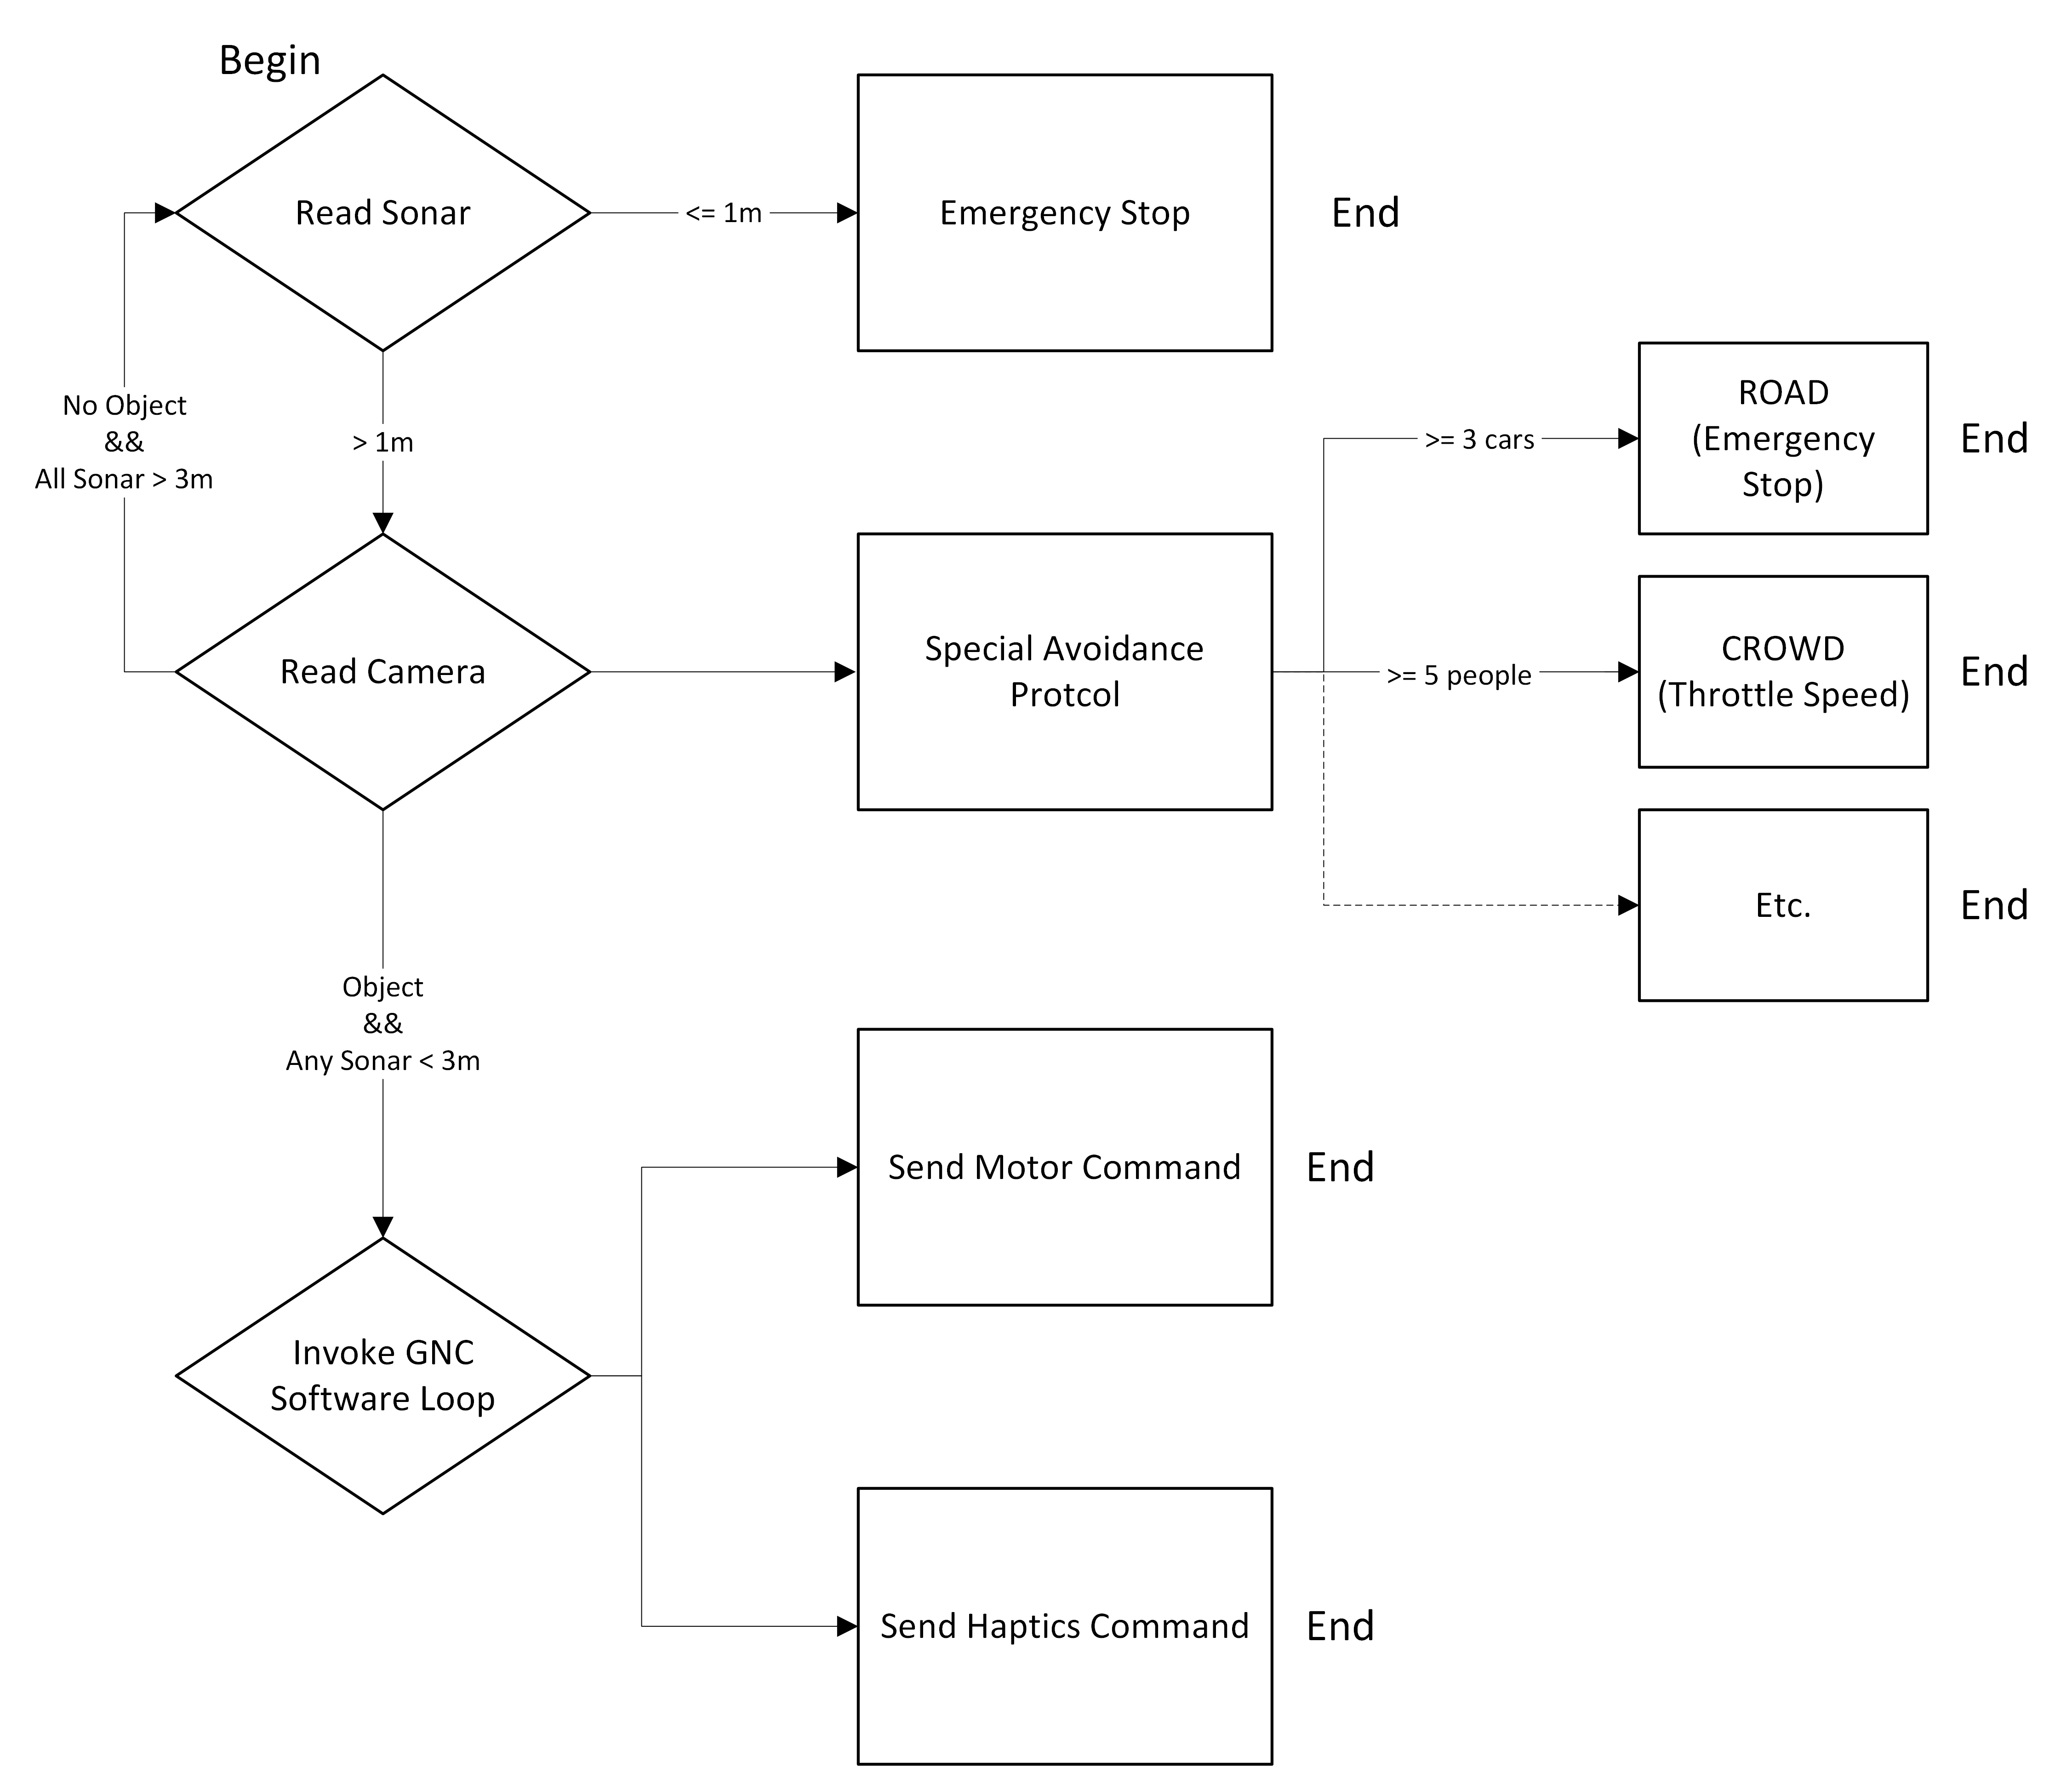
\includegraphics[width=1.0\textwidth]{./Images/Polite-Mobile-Obstacle-Avoidance-Flowchart.png}
	\caption{\label{fig:Polite-Mobile-Obstacle-Avoidance-Flowchart}Polite Mobile Obstacle Avoidance Flowchart}
\end{figure}

\subsection{Guidance, Navigation, and Control Software}
\noindent The block titled "invoke GNC software loop" seen in figure \ref{fig:Polite-Mobile-Obstacle-Avoidance-Flowchart} illustrates the softwre \\  does ... [TOBYBOT GET IN HERE CHIEF KEEF] \\


\noindent GNC situation, tilt (attitude) using IMU, (incline decline), velocity and position solutions, ESP32 source code GitHub (hc-sr04.c luna.c haptic.c audio.c motor.c ip.c avoid.c), motor commands calculation. \\


\subsection{Object Detection}
\noindent The computer vision aspect of our software is very straight forward. The Arduino IDE contains example code for each board file and has an example of an object detection algorithm for the AMB-82 board. To implement this for our purposes, we maintained the YOLO4 Tiny model configuration, the already existing class list for the objects to be detected, and the main loop to extract this data from the algorithm. \\

\noindent While we were able to utilize the example code to help in getting started, there was additional functionality needed to properly fit our purposes. The first of these was implementing WiFi and UDP communication on the board. After doing such, we used a while loop to wait for the ESP32 to assert a transmit flag and once received, the AMB-82 board would complete an object detection run and transmit the data to the ESP32. \\

\subsection{Serial Interface}

\subsection{Motor Control Software}


\noindent [UML CLASS DIAGRAM HERE]\\